% Presentation for second lab.
%
% Copyright (C) 2011  Vladimir Rutsky <altsysrq@gmail.com>
%
% This work is licensed under a Creative Commons Attribution-ShareAlike 3.0
% Unported License. See <http://creativecommons.org/licenses/by-sa/3.0/>
% for details.

\documentclass[utf8]{beamer}
%\documentclass[utf8,handout]{beamer}
\usepackage[russian]{babel}

% \dif, \del{}, \cbr{}, \sbr.
\usepackage{commath}

% Pseudocode as in Cormen book.
\usepackage{clrscode}

% Убирает меню навигации по слайдам.
\setbeamertemplate{navigation symbols}{}

% Футер: номер слайда / общее число слайдов.
%\setbeamertemplate{footline}
%{\centerline{\insertframenumber/\inserttotalframenumber}}

% Футер: Автор, номер слайда
%\setbeamertemplate{footline}{\hspace*{.5cm}\scriptsize{\insertauthor
%\hspace*{50pt} \hfill\insertframenumber\hspace*{.5cm}}}

\defbeamertemplate*{footline}{my split theme}
{%
  \leavevmode%
  \hbox{\begin{beamercolorbox}[wd=.5\paperwidth,ht=2.5ex,dp=1.125ex,leftskip=.3cm plus1fill,rightskip=.3cm]{author in head/foot}%
    \usebeamerfont{author in head/foot}\insertshortauthor
  \end{beamercolorbox}%
  \begin{beamercolorbox}[wd=.4\paperwidth,ht=2.5ex,dp=1.125ex,leftskip=.3cm,rightskip=.3cm]{title in head/foot}%
    \usebeamerfont{title in head/foot}\insertshorttitle
  \end{beamercolorbox}%
  \begin{beamercolorbox}[wd=.1\paperwidth,ht=2.5ex,dp=1.125ex,leftskip=.3cm,rightskip=.3cm plus1fil]{title in head/foot}%
    \usebeamerfont{title in head/foot}\insertframenumber/\inserttotalframenumber
  \end{beamercolorbox}}%
  \vskip0pt%
}

\mode<presentation>
{
  \usetheme{Madrid}
}

\mode<handout>
{
  \usetheme{Madrid}

  \usepackage{pgfpages}
  \pgfpagesuselayout{2 on 1}
}


\DeclareMathOperator*{\argmax}{\arg\!\max}
\DeclareMathOperator*{\argmin}{\arg\!\min}

\title[Оценка параметров случайного процесса]{Оценка параметров модели случайного процесса нагрузки сервера, обрабатывающего заявки}
\author{Владимир Руцкий, 5057/12}
\institute[СПбГПУ]{Санкт-Петербургский государственный политехнический университет}
\date{14 июня 2011}

% Показывает план перед каждой сабсекцией.
%\AtBeginSubsection[]
%{
%  \begin{frame}<beamer>
%  \frametitle{План презентации}
%  \tableofcontents[currentsection,currentsubsection]
%  \end{frame}
%}

\begin{document}

\begin{frame}
\titlepage
\end{frame}


\begin{frame}
\frametitle{План презентации}
\tableofcontents
\end{frame}


\section{Постановка задачи}
\begin{frame}{Постановка задачи}
\begin{block}{Сервер}
  \begin{itemize}
    \item Сервер обрабатывает поступающие заявки
    \item Для обработки заявки используются ресурсы сервера
      \begin{itemize}
        \item Количество используемых ресурсов сервера~--- загрузка сервера ~--- скалярная величина, например процессорное время
      \end{itemize}
  \end{itemize}
\end{block}

\begin{block}{Задача}
  Дан лог загрузки сервера. 
  Необходимо:
  \begin{enumerate}
    \item идентифицировать моменты поступления заявок,
    \item оценить:
      \begin{itemize}
        \item интенсивность поступления заявок,
        \item загрузку сервера в фоновом режиме,
        \item использование ресурсов сервера для обработки одной заявки
      \end{itemize}
  \end{enumerate}
\end{block}
\end{frame}


\begin{frame}{Математическая модель (1)}
Загрузка сервера~--- случайный процесс $X(t)\colon \mathbb{R} \rightarrow \mathbb{R}$
\begin{block}{Фоновая загрузка сервера}
  Сумма постоянной загрузки и винеровского процесса (шум): 
  $$B(t) = m + \sigma \mathcal{W}(t)$$
\end{block}
\begin{block}{Загрузка сервера при обработке заявки}
  Заявка, поступившая в $t=t_c$, увеличивает загрузку сервера на:
  $$K_{t_c}(t) = \mathcal{N}(m_c, \sigma_c^2) \cdot \mathrm{I}(t - t_c) \cdot 
    e^{-\lambda_c(t - t_c)}$$
  {\footnotesize $\mathrm{I}(x) = \left\{
    \begin{array}{rl}
      0, & x < 0 \\
      1, & x \geqslant 0
    \end{array}\right.$~--- Функция Хевисайда}
\end{block}
\end{frame}


\begin{frame}{Математическая модель (2)}
$T_c = \cbr{ t_{c_1}, \ldots, t_{c_R} }$~--- 
множество моментов времени, когда поступили заявки 
(всего $R$ заявок за время наблюдения за сервером)
\begin{block}{Интенсивность поступления заявок}
  Интервал времени между поступлением двух последовательных заявок распределён экспоненциально:
  $$(t_{c_i} - t_{c_{i-1}}) \sim \mathrm{Exp}(\lambda)$$
\end{block}
\begin{block}{Общая загрузка сервера}
  $$X(t) = B(t) + \sum\limits_{t_c \in T_c}K_{t_c}(t)$$
\end{block}
\begin{block}{Перейдём к дискретному случайному процессу}
  $$X(t_i), \quad t_i = t_0 + i \cdot \Delta t \quad 
    (t_0 \mathrm{\text{ и }} \Delta t \mathrm{\text{ даны}})$$
\end{block}
\end{frame}


\begin{frame}{Входные данные}
\begin{block}{Лог загрузки сервера}
  Траектория $X(t_i)\colon \cbr{ x_i \ \vert\ i = 1, \ldots, N }$
\end{block}
Считаем, что $\Delta t$ достаточно мало и $t_{c_j} = t_0 + i \cdot \Delta t$~---
заявки поступили в некоторые наблюдаемые моменты времени $t_i.$

Рассматривается случай $t_0 = 0$
\end{frame}


\begin{frame}{Задача}
\begin{block}{Задача}
  По траектории $X(t_i)$ 
  \begin{enumerate}
    \item идентифицировать моменты поступления заявок,
    \item оценить параметры модели:
      \begin{itemize}
        \item $m, \sigma$~--- параметры фоновой загрузки,
        \item $\lambda$~--- интенсивность поступления заявок,
        \item $m_c, \sigma_c, \lambda_c$~--- параметры загрузки сервера при обработке заявок
      \end{itemize}
  \end{enumerate}
\end{block}
\end{frame}


\section[$\lambda_c \approx 0$]{Решение в случае бесконечного времени обработки заявки}
\begin{frame}{Случай бесконечного времени обработки заявки}
\begin{block}{$\lambda_c \approx 0$}
  При поступлении заявки в момент времени $t_c$ загрузка сервера увеличивается на 
  $\Delta x \sim \mathcal{N}(m_c, \sigma_c)$

  $$K_{t_c}(t) = \mathcal{N}(m_c, \sigma_c^2) \cdot \mathrm{I}(t - t_c)$$
\end{block}
\end{frame}


\begin{frame}{Разностный аналог производной}
\begin{block}{$\dif X(t)$}
  Рассмотрим ненормированный разностный аналог производной:
  $$\dif X(t) = X(t) - X(t - \Delta t)$$
\end{block}
\begin{block}{$\dif X(t)$ в момент времени поступления заявки $t_c$}
  $$\dif X(t_c) = \mathcal{N}(m_c, \sigma^2 \Delta t + \sigma_c^2)$$
  (при условии, что в момент времени $(t_c - \Delta t)$ заявки не было)
\end{block}
\begin{block}{$\dif X(t)$ в момент времени отсутствия заявок $t$}
  $$\dif X(t) = \mathcal{N}(0, \sigma^2 \Delta t)$$
  (при условии, что в момент времени $(t - \Delta t)$ заявки не было)
\end{block}
\end{frame}


\subsection{Итеративный метод}
\begin{frame}{Итеративный метод идентификации заявок (1)}
Предположим, что в отрезке времени $\sbr{t_k, t_{k+n}}$ 
не поступило ни одной заявки.

Тогда $\dif x_k, \dots, \dif x_{k+n}$~--- наблюдения 
$\mathcal{N}(0, \sigma^2 \Delta t) = \dif X(t).$

Оценим $\sigma^2$ по $\sbr{x_k, x_{k+n}}$:
$$\widehat{\sigma}^2 \Delta t = 
    \frac{1}{n-1}
        \sum\limits_{i=1}^n ((x_{k+i} - x_{k+i-1}) - 0)^2$$

\begin{block}{Гипотеза $H_0$}
  В отрезке времени $\sbr{t_{k+n}, t_{k+n} + \Delta t}$ не поступило ни 
  одной заявки
\end{block}
\begin{block}{Критерий принятия $H_0$ с уровнем значимости $\alpha$}
Разность значений наблюдений $(x_{k+n+1}-x_{k+n})$
лежит в $\del{1 - \alpha}$ квантиле
нормального распределения $\mathcal{N}(0, \widehat{\sigma}^2 \Delta t)$:
$$
H_0 \  \mathrm{\text{принимается}} \iff
        (x_{k+n+1}-x_{k+n}) < 
	    \mathcal{N}_{1 - \alpha}
$$
\end{block}
\end{frame}


\begin{frame}{Итеративный метод идентификации заявок (2)}
\begin{block}{Алгоритм итеративной идентификации первой заявки}
  \begin{codebox}
  \Procname{$\proc{Find-Request-Index}
      \del{D = \cbr{\dif x_{i + \mathrm{offset}}}, n, \alpha}$}
  \li \For $k \gets n$ \To $\id{length}[D] - 1$
  \li \Do
        $\id{H_0-criterion} \gets
          \proc{Build-H0-Criterion}\del{D[1 \twodots k], \alpha}$
  \li   \If \kw{not} $\id{H_0-criterion}(D[k+1])$
  \zi   \Then
          \Comment $(k+1)$-й выброс отвергает $H_0 \implies$ заявка      
  \li     \Return $k+1$
        \End
  \li   \End
  \li \Return 0 \Comment Заявка не обнаружена
  \end{codebox}
\end{block}
\end{frame}


\begin{frame}{Итеративный метод идентификации заявок (3)}
\begin{block}{Алгоритм итеративной идентификации всех заявок}
  \begin{codebox}
  \Procname{$\proc{Find-Requests-Iterative}
      \del{D=\cbr{\dif x_i}, n, \alpha}$}
  \li $\widehat{T_c} \gets \varnothing$
  \li $\id{idx} \gets 0$ \Comment Индекс последней идентифицированной заявки
  \li \While \const{true}
  \li \Do
        \Comment Находим индекс следующей заявки
  \li   $\id{idx} \gets \proc{Find-Request-Index}
            \del{D\sbr{\id{idx} + 1 \twodots \id{length}[D]}, 
            n, \alpha}$
  \li   \If $\id{idx} \neq 0$
  \li   \Then
          $\widehat{T_c} \gets \widehat{T_c} \cup \cbr{t_{idx}}$
  \li   \Else
          \Return $\widehat{T_c}$
        \End
      \End
  \end{codebox}
\end{block}
\end{frame}


\begin{frame}{Оценка параметров модели}

\begin{block}{Интенсивность поступления заявок}
$$\widehat{\lambda} = 
    \frac{1}{|\widehat{T_c}|} 
        \sum\limits_{i=1}^{|\widehat{T_c}|} (t_{c_{i+1}} - t_{c_i})$$
\end{block}
\begin{block}{Параметры фоновой загрузки}
$$
  \widehat{m} = \frac{1}{K-1} \sum\limits_{i=1}^{K-1} x_i, \quad
  \widehat{\sigma}^2 = 
      \frac{1}{K-2} \sum\limits_{i=1}^{K-1} \del{x_i - \widehat{m}}^2, \quad
  K = t_{c_1} / \Delta t
$$
\end{block}
\begin{block}{Параметры загрузки при обработке заявок}
$$
  \widehat{m_c} = \frac{1}{\envert{T_c}} \sum\limits_{t_c \in T_c} 
      \dif x_{t_c / \Delta t}, \quad
  \widehat{\sigma}^2 \Delta t + \widehat{\sigma_c}^2 = 
      \frac{1}{\envert{T_c} - 1} \sum\limits_{t_c \in T_c}
      \del{\dif x_{t_c / \Delta t} - \widehat{m_c}}^2
$$
\end{block}
\end{frame}


\subsection[EM-алгоритм]{Оценивание EM-алгоритмом}
\begin{frame}{EM-алгоритм. Скрытые случайные величины}
\begin{block}{$Z_i$}
  Введём скрытые случайные величины $Z_i, \quad i=1,\ldots,N$
  \begin{itemize}
    \item $Z_i = 1,$ если в момент времени $t_i$ поступила заявка,
    \item $Z_i = 2,$ если в момент времени $t_i$ не поступила заявка
  \end{itemize}
  Количество поступивших за время наблюдения заявок~--- случайная величина, 
  распределённая по закону Пуассона $\mathcal{P}(\lambda).$

  $\mathcal{P}(\lambda)$ можно аппроксимировать Биномиальным законом 
  $\mathcal{B}(N, \tau).$

  $\implies$ $Z_i$ можно считать распределённой по закону Бернулли.

  $\mathbf{P}(Z_i=1) = \tau_1$, $\mathbf{P}(Z_i=2) = \tau_2 = 1 - \tau_1$
\end{block}

$$
\begin{array}{rclcll}
\dif X(t_i) \vert (Z_i = 1) &\sim& \mathcal{N}(\mu_1, \sigma_1^2) &=& 
  \mathcal{N}(m_c, \sigma^2 \Delta t + \sigma_c^2), &
  \quad (t_i \in T_c), \\
\dif X(t_i) \vert (Z_i = 2) &\sim& \mathcal{N}(\mu_2, \sigma_2^2) &=& 
  \mathcal{N}(0, \sigma^2 \Delta t), &
  \quad (t_i \notin T_c).
\end{array}
$$

Введём обозначения: 
$\theta = (\tau_1, \tau_2, \mu_1, \mu_2, \sigma_1^2, \sigma_2^2),$
$\mathbf{\dif x} = (\dif x_1, \ldots, \dif x_N),$
$\mathbf{z} = (z_1, \ldots, z_N)$
\end{frame}


\begin{frame}{EM-алгоритм. Построение функции правдоподобия}
\begin{block}{Функция правдоподобия}
  $$
  L(\theta; \dif \mathbf{x}, \mathbf{z}) = 
    \mathbf{P}(\dif \mathbf{x}, \mathbf{z} \vert \theta) = 
    \prod\limits_{i=1}^{N} \sum\limits_{j=1}^2 
      \mathbb{I}(z_i=j) \, \tau_j \, f(\dif x_i,\mu_j,\sigma_j^2),
  $$

{\footnotesize
$\mathbb{I}(\mathrm{expr}) = \left\{
  \begin{array}{rl}
    0, & \mathrm{expr} = \mathrm{False} \\
    1, & \mathrm{expr} = \mathrm{True}
  \end{array}\right.$~--- функция индикатор

$f(x, \mu, \sigma^2) = 
    \frac{1}{\sqrt{2 \pi \sigma^2}} e^{-\frac{(x - \mu)^2}{2 \sigma^2}}$~---
плотность нормального распределения
}
\end{block}

В экспоненциальной форме:
{\small
$$
L(\theta; \dif \mathbf{x}, \mathbf{z}) =
  \exp \cbr{ \sum\limits_{i=1}^{N} \sum\limits_{j=1}^2 
    \mathbb{I}(z_i=j) \sbr{
      \log \tau_j - 
      \frac{1}{2}\log(2\pi) -
      \log(\sigma_j) -
      \frac{(\dif x_i - \mu_j)^2}{2 \sigma_j^2}}}
$$}
\end{frame}


\begin{frame}{EM-алгоритм}
\begin{block}{EM-алгоритм}
\begin{codebox}
\Procname{$\proc{EM-Algorithm}$()}
\li $\theta \gets \proc{Estimate-Initial-Parameters}()$
\li \While \const{true}
\li \Do
      $\theta_{\mathrm{next}} \gets \proc{M-Step}(\proc{E-Step}())$
\li   \If $\envert{\theta - \theta_{\mathrm{next}}} < \varepsilon$
\li   \Then
        \Return $\theta$
\li   \Else
        $\theta \gets \theta_{\mathrm{next}}$
      \End
    \End
\end{codebox}
\end{block}
\end{frame}


\begin{frame}{EM-алгоритм. Оценивание начальных параметров}
\begin{block}{$\tau_j$}
$$
\tau_j^{(0)} = 0.5, \quad j=1,2
$$
\end{block}
\begin{block}{$\mu_j$}
Построим полигон частот $\dif x_i$.
В качестве $\mu_1^{(0)}$ возьмём последний локальный максимум частот,
а в качестве $\mu_2^{(0)}$~--- первый
\end{block}
\begin{block}{$\sigma_j$}
$$\sigma_j^{(0)} = \frac{1}{3}\del{\mu_1^{(0)} - \mu_2^{(0)}}, \quad j=1, 2$$
\end{block}
\end{frame}


\begin{frame}{EM-алгоритм. E-шаг}
\begin{block}{Условная вероятность принадлежности $i$-го наблюдения}
По Т.~Байеса:
\begin{eqnarray*}
  T_{j,i}^{(k)} 
    &=& \mathbf{P}\del{Z_i = j \vert \dif X(t_i) = \dif x_i; \theta^{(k)}} = \\
    &=& 
    \frac{\tau_j^{(k)} \cdot f\del{\dif x_i; \mu_j^{(k)}, \sigma_j^{(k)}}}
         {\tau_1^{(k)} \cdot f\del{\dif x_i; \mu_1^{(k)}, \sigma_1^{(k)}} + 
         {\tau_2^{(k)} \cdot f\del{\dif x_i; \mu_2^{(k)}, \sigma_2^{(k)}}}}
\end{eqnarray*}
\end{block}
\begin{block}{Математическое ожидание логарифма функции правдоподобия}
\begin{eqnarray*}
  Q\del{\theta \vert \theta^{(k)}} 
    &=& 
    \mathbf{E}\sbr{\log L(\theta; \dif \mathbf{x}, \mathbf{z})} = \\
    &=& \sum\limits_{i=1}^{N} \sum\limits_{j=1}^2
      T_{j,i}^{(k)} 
        \sbr{
          \log \tau_j - 
          \frac{1}{2}\log(2\pi) -
          \log(\sigma_j) -
          \frac{(\dif x_i - \mu_j)^2}{2 \sigma_j^2}
        }
\end{eqnarray*}
\end{block}
\end{frame}


\begin{frame}{EM-алгоритм. M-шаг}
\begin{block}{Максимизация $Q\del{\theta \vert \theta^{(k)}}$}
$$
\theta^{(k+1)} = \argmax\limits_{\theta} Q\del{\theta \vert \theta^{(k)}}.
$$
$$
\tau_j^{(k+1)} = \frac{1}{n} \sum\limits_{i=1}^{N} T_{j,i}^{(k)},\quad
\mu_j^{(k+1)} = \frac
  {\sum\limits_{i=1}^{N} T_{j,i}^{(k)} \dif x_i}
  {\sum\limits_{i=1}^{N} T_{j,i}^{(k)}},
$$
$$
\sigma_j^{(k+1)} = \frac
  {\sum\limits_{i=1}^{N} T_{j,i}^{(k)} \del{\dif x_i - \mu_j^{(k+1)}}^2}
  {\sum\limits_{i=1}^{N} T_{j,i}^{(k)}}
$$
\end{block}
\end{frame}


\begin{frame}{EM-алгоритм. Получение оценок параметров модели}
\begin{block}{Оценка $\sigma^2$, $m_c$, $\sigma_c$}
$$
  \widehat{m_c} = \mu_1, \quad 
  \widehat{\sigma}^2 = \frac{\sigma_2^2}{\Delta t}, \quad
  \widehat{\sigma_c}^2 = \sigma_1^2 - \sigma_2^2
$$
\end{block}
\begin{block}{Оценка времени поступления заявок}
$$\widehat{T_c} = \cbr{t_i \quad i=1,\ldots,N\ \vert\ 
    T_{1,i}^{(k)} > T_{2,i}^{(k)}}$$
\end{block}

Оценки $m$ и $\lambda$ получаем так же, как в итеративном методе
\end{frame}


\section[$\lambda_c \gg 0$]{Решение в случае конечного времени обработки заявки}
\begin{frame}{Случай конечного времени обработки заявки}
\begin{block}{$\lambda_c \gg 0$}
\begin{eqnarray*}
X(t) 
  &=& B(t) + \sum\limits_{t_c \in T_c}K_{t_c}(t) = \\
  &=& m + \sigma \mathcal{W}(t) + \sum\limits_{t_c \in T_c}
    \mathcal{N}(m_c, \sigma_c^2) \cdot \mathrm{I}(t - t_c) \cdot 
    e^{-\lambda_c(t - t_c)}
\end{eqnarray*}
\end{block}
Считаем, что заявки поступают достаточно редко и 
обрабатываются достаточно быстро: 
для каждой заявки предыдущие заявки практически не влияют на уровень
загруженности
\end{frame}


\begin{frame}{Разностный аналог производной}
\begin{block}{$\dif X(t)$ в момент времени поступления заявки $t_c$}
  \begin{eqnarray*}
  \dif X(t_c) 
    & = & X(t_c) - X(t_c - \Delta t) = \\
    & = & \mathcal{N}(m_c, \sigma^2 \Delta t + \sigma_c^2).
  \end{eqnarray*}
  (при условии, что в момент времени $(t_c - \Delta t)$ заявки не было)
\end{block}
\begin{block}{$\dif X(t)$ в момент времени отсутствия заявок $t$}
  \begin{eqnarray*}
  \dif X(t) 
    & = & X(t) - X(t - \Delta t) = \\
    & = & \mathcal{N}(0, \sigma^2 \Delta t) + 
        \mathcal{N}(m_c, \sigma_c^2) \cdot 
          \del{e^{-\lambda_c(t - t_c)} - e^{-\lambda_c(t - \Delta t - t_c)}}.
  \end{eqnarray*}
  (при условии, что в момент времени $(t - \Delta t)$ заявки не было)
\end{block}
\end{frame}


%\subsection{Идентификация моментов времени поступления заявок}
\begin{frame}{Идентификация моментов времени поступления заявок}
\begin{enumerate}
\item Построим вариационный для $\dif x_i$:
  $$\dif x_{(1)} \leqslant \dif x_{(2)} \leqslant \ldots 
    \leqslant \dif x_{(N)}.$$
  Приходящие заявки вносят существенно большее изменение уровня загруженности
  ресурсов сервера, чем фоновая нагрузка

  $\implies$ все наблюдения $\dif X(t_c)$ находятся в правой части ряда.

\item Используя итеративный метод для идентификации заявок 
$\proc{Find-Request-Index},$
найдём границу $k$ наблюдений $\dif X(t_c)$ в вариационном ряде:
$$
  \dif x_{(i)} \sim \dif X(t_c), \quad i \geqslant k.
$$

\item По границе $k$ выделим наблюдения из $\widehat{T_c}$
\end{enumerate}
\end{frame}


\subsection[МНК]{Метод наименьших квадратов}
\begin{frame}{Метод наименьших квадратов (1)}
\begin{block}{В моменты времени между поступлениями заявок $\sbr{t_k, t_{k+n}}$}
\begin{eqnarray*}
\dif X(t) 
  & = & \mathcal{N}(0, \sigma^2 \Delta t) + 
      \mathcal{N}(m_c, \sigma_c^2) \cdot 
        \del{e^{-\lambda_c(t - t_c)} - e^{-\lambda_c(t - \Delta t - t_c)}} \\
  & = & \del{
      \mathcal{N}(0, \sigma^2 \Delta t) + 
      \mathcal{N}(0, \sigma_c^2) \cdot 
        \del{e^{-\lambda_c(t - t_c)} - e^{-\lambda_c(t - \Delta t - t_c)}}} +\\
      && m_c \cdot 
        \del{e^{-\lambda_c(t - t_c)} - e^{-\lambda_c(t - \Delta t - t_c)}}
\end{eqnarray*}
\end{block}
\end{frame}


\begin{frame}{Метод наименьших квадратов (2)}
\begin{block}{Метод наименьших квадратов}
\begin{eqnarray*}
\del{m_c, \lambda_c} 
  & = & \argmin\limits_{m_c,\ \lambda_c} S(m_c, \lambda_c) = \\
  & = & \argmin\limits_{m_c,\ \lambda_c} \sum\limits_{i=1}^{n} 
    \del{\dif x_i - m_c \cdot 
      \del{e^{-\lambda_c(t_i - t_k)} - 
           e^{-\lambda_c(t_i - \Delta t - t_k)}}}^2
\end{eqnarray*}
\end{block}
$S(m_c, \lambda_c)$ выпукла вниз на интересущей для анализа области~---
используем численный метод минимизации (метод покоординатного спуска)
\end{frame}


\begin{frame}{Оценка параметров фоновой загрузки}
$m$ и $\sigma$ оцениваются так же, как в итеративном методе
\end{frame}


\section{Результаты работы}
\begin{frame}{Результаты работы (1)}
\begin{figure}
   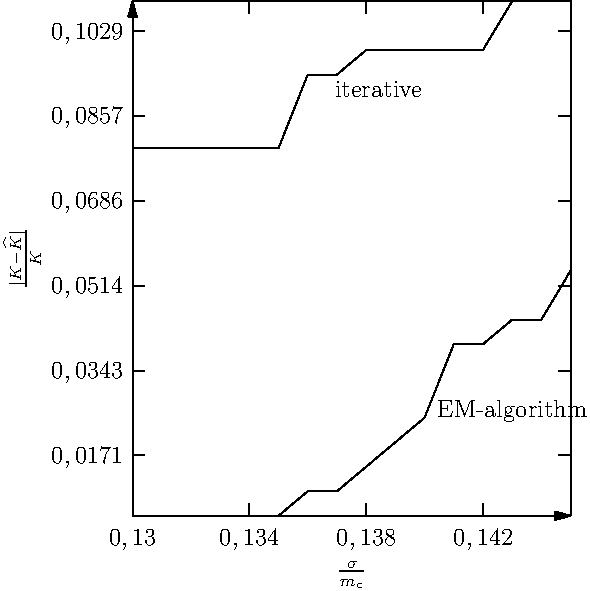
\includegraphics[height=7.5cm]{../../data/K_of_sigma.pdf}
\end{figure}
\end{frame}


\begin{frame}{Результаты работы (2)}
\begin{figure}
   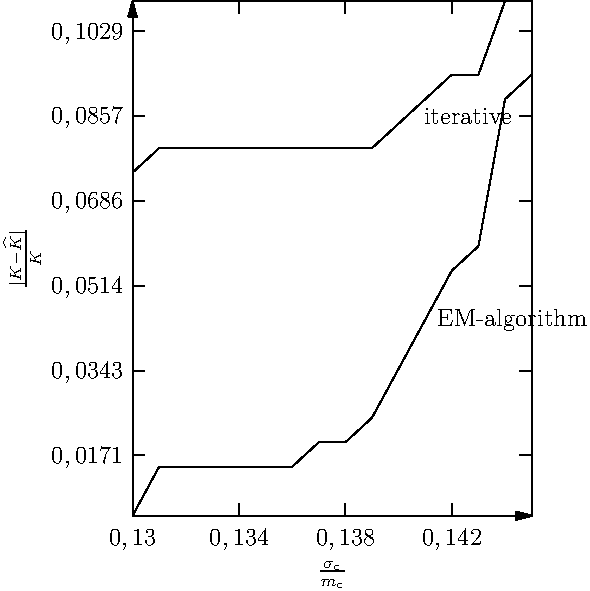
\includegraphics[height=7.5cm]{../../data/K_of_sigma_c.pdf}
\end{figure}
\end{frame}


\begin{frame}{Результаты работы (3)}
\begin{figure}
   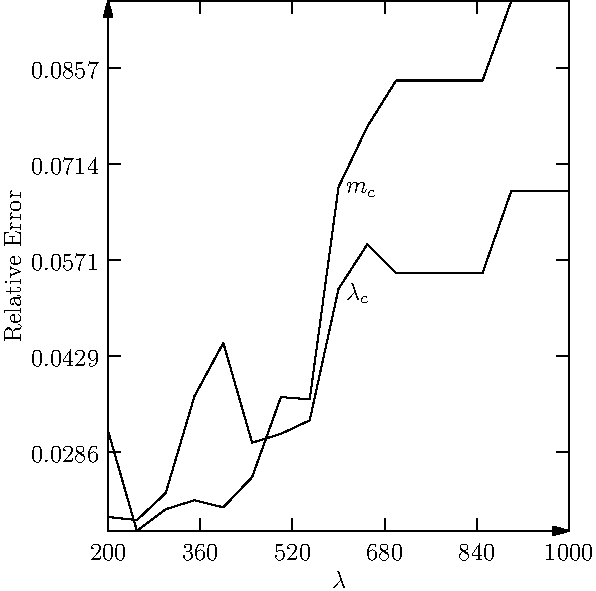
\includegraphics[height=7.5cm]{../../data2/gen_params_stats_lambda.pdf}
\end{figure}
\end{frame}


\begin{frame}{Результаты работы (4)}
\begin{figure}
   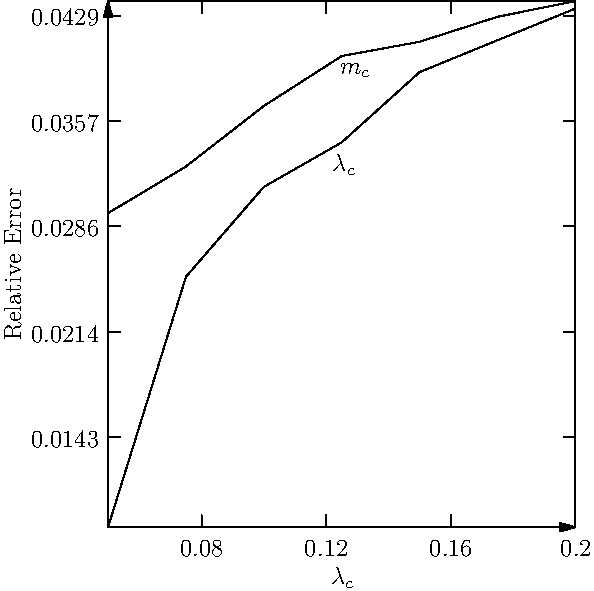
\includegraphics[height=7.5cm]{../../data2/gen_params_stats_lambda_signal.pdf}
\end{figure}
\end{frame}


\begin{frame}{Результаты работы (5)}
\begin{figure}
   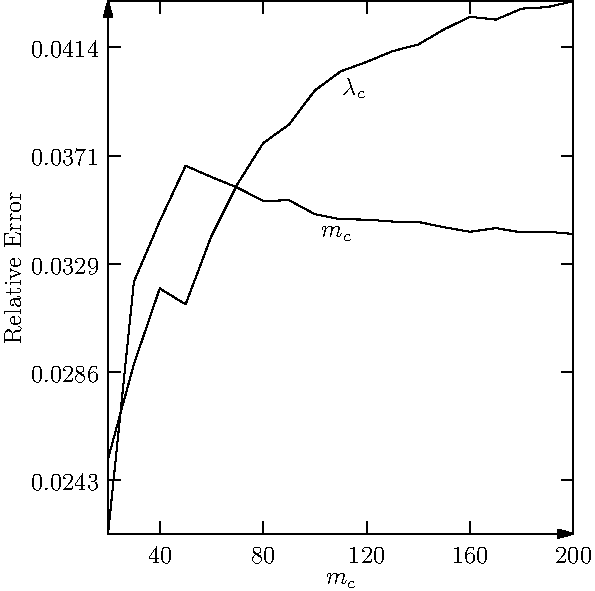
\includegraphics[height=7.5cm]{../../data2/gen_params_stats_m_signal.pdf}
\end{figure}
\end{frame}


\begin{frame}{Результаты работы (6)}
\begin{figure}
   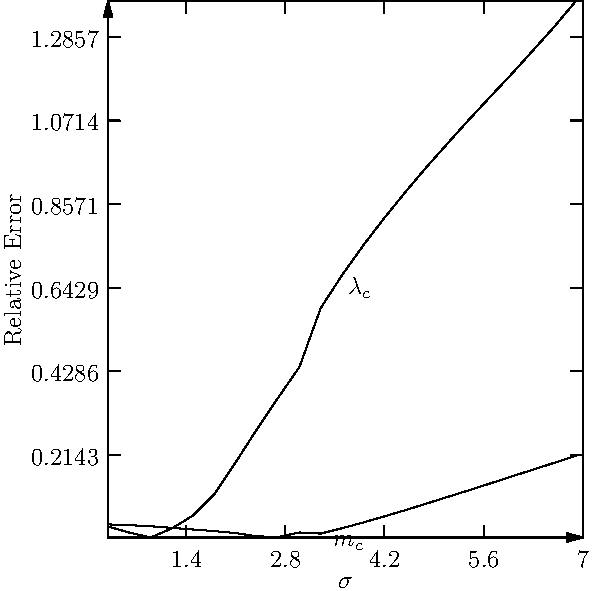
\includegraphics[height=7.5cm]{../../data2/gen_params_stats_sigma.pdf}
\end{figure}
\end{frame}


\begin{frame}{Результаты работы (7)}
\begin{figure}
   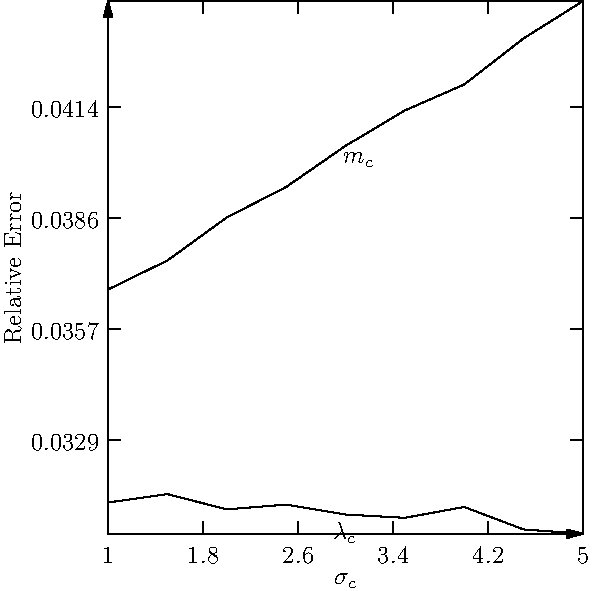
\includegraphics[height=7.5cm]{../../data2/gen_params_stats_sigma_signal.pdf}
\end{figure}
\end{frame}


%\begin{frame}{Выводы}
%\end{frame}


%\begin{frame}{Список литературы}
%  \begin{thebibliography}{10}
%    \bibitem{ivchmed2010matstat}[Ивченко, 2010] Г.\,И.~Ивченко, Медведев~Ю.\,И.
%    \emph{{Введение в математическую статистику}}
%    %\newblock A problem we should try to solve before the ISPN ’43 deadline,
%    %\newblock \emph{Letter to Leonhard Euler}, 1742.
%  \end{thebibliography}
%\end{frame}


\end{document}

% vim: set ts=2 sw=2 et:
